% ======================================================================
% Relatório de Pesquisa (Iniciação Científica) — UFABC
% Tema: Iridologia sob Lentes Científicas: Avaliação Crítica com ML
% ======================================================================

\documentclass[12pt,a4paper]{article}
\usepackage{graphicx}
% ---------------------- Pacotes ----------------------
\usepackage[utf8]{inputenc}
\usepackage[T1]{fontenc}
\usepackage[portuguese]{babel}

\usepackage{setspace}
\usepackage{geometry}
\usepackage{tabularx}
\geometry{a4paper, top=3cm, bottom=2.5cm, left=3cm, right=2.5cm}

\usepackage{graphicx}
\graphicspath{{./imagens/}}
\usepackage{float}

\usepackage{amsmath, amssymb}
\usepackage{siunitx}
\sisetup{
  mode = match,
  propagate-math-font = true,
  reset-math-version = false,
  reset-text-family = false,
  reset-text-series = false,
  reset-text-shape = false,
  text-family-to-math = true,
  text-series-to-math = true
}

\usepackage{booktabs}
\usepackage{multirow}
\usepackage{array}

\usepackage{fancyhdr}
\setlength{\headheight}{14pt}

% Natbib em autor--ano (compatível com \bibitem[Autor(ano)]{...})
\usepackage[authoryear, round, sort]{natbib}

% hyperref por último (boa prática)
\usepackage[bookmarks=true, colorlinks=true, linkcolor=blue, citecolor=blue, urlcolor=blue]{hyperref}

\usepackage{indentfirst}
\setlength{\parindent}{1.25cm}
\setlength{\parskip}{0.2cm}

% ---------------------- Cabeçalho/Rodapé ----------------------
\pagestyle{fancy}
\fancyhf{}
\lhead{\small UFABC — Programa de Iniciação Científica}
\rhead{\small Relatório de Pesquisa}
\cfoot{\thepage}

% ---------------------- Metadados ----------------------
\title{\textbf{Relatório de Pesquisa (Iniciação Científica)}\\
\large Iridologia sob Lentes Científicas: Avaliação Crítica com Aprendizado de Máquina\\
\vspace{0.2cm}\normalsize (Ênfase: alegações diagnósticas para diabetes mellitus tipo 2)}
\date{Santo André, 18 de dezembro de 2025}

% ----------------------------------------------------------------------
\begin{document}

\hypersetup{pageanchor=false}

% ====================== Capa ======================
\begin{titlepage}
\begin{center}

{\large \textbf{UNIVERSIDADE FEDERAL DO ABC}}\\[0.25cm]
{\large \textbf{PRÓ REITORIA DE PESQUISA}}\\[1.2cm]

{\normalsize \textbf{Relatório Parcial de Iniciação Científica referente ao Edital: 01/2025}}\\[0.6cm]
\end{center}
\\
\textbf{Nome do aluno:} Vinicius Sedrim. \\
\textbf{Assinatura do aluno:}\\\\\\\\\\\\
\textbf{Nome do orientador:} Vladimir Emiliano Moreira Rocha. \\
\textbf{Assinatura do orientador:} \\\\\\\\\\\\
\textbf{Título do projeto:} Iridologia sob Lentes Científicas: Avaliação Crítica com Aprendizado de Máquina. \\
\textbf{Palavras-chave do projeto:} Iridologia; Medicina Alternativa; Visão Computacional; Aprendizado de Máquina. \\
\textbf{Área do conhecimento do projeto:} Ciência da Computação. \\
\textbf{Bolsista:} Sim. CNPq. \\

\begin{center}
\vfill
{\normalsize Santo André}\\
{\normalsize 10 de março de 2026}

\end{center}
\end{titlepage}

% ====================== Resumo ======================
\begin{abstract}
Este projeto conduz uma \textbf{avaliação crítica, científica e reprodutível} de alegações de que padrões observáveis na íris possam sustentar inferência de \textbf{diabetes mellitus tipo 2 (DM2)}, no contexto da literatura de iridologia e de estudos recentes em \textit{machine learning} (ML). Estudos clínicos clássicos e revisões sistemáticas relatam \textbf{baixa acurácia} e \textbf{baixa confiabilidade} da iridologia quando avaliada sob protocolos controlados. Em contraste, trabalhos em ML frequentemente reportam alto desempenho ao classificar DM2 a partir de imagens da íris, porém com limitações metodológicas recorrentes, incluindo amostras reduzidas, heterogeneidade de protocolos, risco de \textit{data leakage} (inclusive por identidade) e ausência de testes sistemáticos de robustez.

Neste relatório, descrevem-se o problema, os objetivos, a base teórica e uma \textbf{metodologia auditável} orientada à \textbf{generalização} e ao \textbf{controle de viés}. O protocolo emprega: (i) particionamento \textit{person-based} (separação por indivíduo) para mitigar vazamento por identidade; (ii) validação cruzada estratificada e reexecução completa do \textit{pipeline} (segmentação, normalização e classificação); (iii) avaliação por múltiplas métricas (Acc, Sens, Esp, Prec e F1); (iv) análises de estabilidade sob reamostragens/\textit{folds} e diferentes sementes; e (v) testes de sensibilidade a transformações fotométricas. Resultados preliminares indicam desempenho elevado e consistente em diferentes classificadores sob controle \textit{person-based}, com manutenção do desempenho sob perturbações fotométricas moderadas. Análises locais (setores angulares e ROI pancreática em malha \(12\times 12\)) são tratadas como \textbf{exploratórias} e interpretadas como \textbf{hipóteses candidatas}, cuja validade exige verificação confirmatória com controles para múltiplas comparações e testes adicionais de generalização.
\end{abstract}


\tableofcontents
\newpage

\hypersetup{pageanchor=true}
\pagenumbering{arabic}
\setcounter{page}{1}

\doublespacing

% ====================== Introdução ======================
\section{Introdução}
A iridologia é uma prática que afirma ser possível identificar indícios de saúde e doença a partir de padrões observáveis na íris, como variações de textura, coloração, sulcos, anéis e marcas. Em sua forma mais difundida, utiliza \textit{mapas iridológicos} que associam regiões específicas do olho a órgãos e sistemas do corpo, sugerindo que alterações locais na íris poderiam refletir disfunções internas \citep{Ernst2000ArchOphthalmol}. Por isso, em alguns contextos, a iridologia é apresentada como proposta complementar de triagem e acompanhamento. Entretanto, quando a prática é apresentada com finalidade \textbf{diagnóstica} (isto é, para inferir doenças de forma confiável), a exigência científica é alta: é necessário demonstrar validade, reprodutibilidade, controle de vieses e desempenho consistente em cenários realistas \citep{AusGovIridology2025}.

Essa exigência se torna ainda mais crítica ao considerar doenças crônicas de grande impacto, como o diabetes mellitus tipo 2 (DM2). O DM2 é uma condição metabólica multifatorial associada a complicações cardiovasculares, renais, neurológicas e oftalmológicas, e cuja progressão pode permanecer silenciosa por longos períodos \citep{WHOdiabetes2024}. Por esse motivo, estratégias de detecção precoce e monitoramento são frequentemente discutidas em saúde pública, especialmente quando envolvem soluções de baixo custo e fácil acesso \citep{WHOdiabetes2024}. Nesse cenário, propostas não invasivas naturalmente ganham espaço --- incluindo ideias que vão desde marcadores fisiológicos validados até hipóteses que ainda carecem de evidência clínica robusta.

A literatura médica clássica, no entanto, apresenta resultados desfavoráveis à iridologia quando avaliada sob protocolos controlados e com critérios diagnósticos objetivos. Estudos clínicos e revisões sistemáticas relatam baixa acurácia e pouca confiabilidade, sugerindo que a prática não sustenta promessas diagnósticas em condições investigadas \citep{Simon1979JAMA, Knipschild1988BMJ, Ernst2000ArchOphthalmol}. Em linha semelhante, avaliações recentes que sintetizam evidências para decisões de saúde pública reforçam a ausência de confiabilidade diagnóstica atribuível à iridologia \citep{AusGovIridology2025}. Esses resultados não apenas questionam a validade do método, mas também indicam um risco prático: interpretações incorretas podem gerar falsa segurança, ansiedade desnecessária ou atraso em diagnóstico clínico adequado.

Paralelamente, o avanço recente de visão computacional e aprendizado de máquina (\textit{machine learning}, ML) traz um elemento novo para esse debate. Modelos modernos podem aprender padrões complexos em imagens, inclusive padrões sutis que não são facilmente percebidos por observadores humanos. Isso reabre uma questão central: existe algum sinal estatístico real nas imagens associado ao DM2? Ou, alternativamente, desempenhos elevados reportados por modelos decorrem de atalhos e artefatos do processo experimental, como diferenças de iluminação e câmera, ruídos de segmentação ou vazamento de dados (\textit{data leakage}), que permitem ao modelo reconhecer identidade (ou características indiretas) em vez de doença \citep{SamantAgarwal2018CMPB}? Assim, métricas altas podem refletir confundidores do \textit{pipeline} e do protocolo de aquisição, e não necessariamente a aprendizagem de um marcador clínico.

Este projeto nasce exatamente desse ponto de tensão: de um lado, uma prática historicamente contestada por estudos clínicos; de outro, resultados em ML que sugerem separabilidade entre grupos (indivíduos com DM2 versus indivíduos controle) \citep{SamantAgarwal2018CMPB}. O objetivo não é confirmar crenças prévias, mas construir um protocolo experimental rigoroso e auditável que permita testar \textbf{as hipóteses típicas de mapeamentos iridológicos} de forma justa. Para isso, adota-se um \textit{pipeline} reprodutível (segmentação, normalização e validação estratificada), métricas completas (incluindo sensibilidade e especificidade) e controles explícitos contra vazamento de dados --- em especial vazamento por identidade, por meio de separação por indivíduo nos particionamentos. Além disso, realizam-se análises locais por região, conectando os experimentos às hipóteses espaciais propostas por mapeamentos iridológicos. Assim, busca-se diferenciar evidência de sinal estatístico de explicações alternativas baseadas em viés metodológico e artefatos, produzindo uma conclusão baseada em resultados replicáveis e critérios de generalização.


% ====================== Problema de Pesquisa ======================
\section{Problema e Questões de Pesquisa}

\subsection{Contexto e motivação do problema}
A iridologia sustenta a hipótese de que a íris contém marcas e padrões que refletiriam condições sistêmicas do organismo, sendo interpretada com apoio de \textit{mapas iridológicos} que associam regiões do olho a órgãos específicos. Em termos científicos, essa hipótese exige evidência empírica forte, pois implica uma relação causal entre características visuais da íris e estados fisiopatológicos internos. Entretanto, a literatura clínica clássica tende a demonstrar baixa confiabilidade diagnóstica e desempenho limitado quando a iridologia é avaliada sob protocolos controlados conduzidos por avaliadores humanos treinados \citep{Simon1979JAMA, Knipschild1988BMJ, Ernst2000ArchOphthalmol}.

Nos últimos anos, o avanço do aprendizado de máquina (ML) e da visão computacional reabriu parcialmente esse debate. Alguns estudos relatam acurácias elevadas para classificar DM2 a partir de imagens da íris, sugerindo a existência de um padrão discriminativo \citep{SamantAgarwal2018CMPB}. Contudo, em aplicações de visão computacional médica, desempenhos elevados podem decorrer de fatores que não correspondem a um marcador clínico legítimo, como \textit{data leakage} (por exemplo, quando o mesmo indivíduo aparece nos conjuntos de treino e teste), viés de aquisição (câmera, iluminação, ambiente), rotulagem imperfeita ou padrões introduzidos pelas próprias etapas de segmentação e normalização \citep{Zech2018}. Na prática, modelos podem aprender \textbf{atalhos estatísticos} (\textit{shortcuts}) que funcionam dentro de um conjunto de dados específico, mas não se sustentam sob condições de generalização.

Dessa forma, o desafio científico central não consiste apenas em obter valores elevados de acurácia, mas em demonstrar que o desempenho observado apresenta propriedades fundamentais de validade empírica, a saber:
(i) é \textbf{reprodutível}, ou seja, mantém-se sob reexecuções do experimento;
(ii) é \textbf{generalizável}, isto é, resiste a novas divisões dos dados e, idealmente, a conjuntos independentes;
(iii) não depende predominantemente de fatores não clínicos, como artefatos e vieses metodológicos;
e (iv) permanece consistente quando hipóteses locais inspiradas por mapas iridológicos são avaliadas.

\subsection{Problema central}
Dadas as controvérsias históricas sobre a iridologia e os riscos metodológicos associados ao uso de ML com imagens, o problema central deste projeto \textbf{não se limita a} valores elevados de acurácia. Ele consiste em avaliar se imagens da íris contêm informação diagnóstica útil para DM2 quando analisadas sob um protocolo experimental rigoroso, com controle explícito de vieses e prevenção de \textit{data leakage}, e se o desempenho observado pode ser considerado reprodutível, robusto e generalizável.

De forma complementar, busca-se determinar se a separabilidade observada entre indivíduos com DM2 e indivíduos controle reflete a presença de um sinal estatístico consistente nas imagens ou se é melhor explicada por limitações do desenho experimental e por artefatos metodológicos.

\subsection{Questões específicas}
As questões de pesquisa que operacionalizam esse problema central são formuladas nos seguintes termos:

\begin{enumerate}
    \item \textbf{Validade global do sinal (íris inteira):} verificar se, ao aplicar um \textit{pipeline} reprodutível (segmentação, normalização e extração de representações) e treinar modelos sob validação cruzada estratificada, o desempenho permanece consistentemente acima de baselines e mantém equilíbrio clinicamente relevante entre sensibilidade e especificidade.

    \item \textbf{Generalização e estabilidade dos resultados:} avaliar se o desempenho observado permanece estável sob:
    \begin{itemize}
        \item variação das sementes aleatórias,
        \item diferentes estratégias de validação,
        \item variações moderadas no pré-processamento,
        \item e, quando possível, aplicação do modelo a conjuntos de dados independentes.
    \end{itemize}
    O objetivo é distinguir entre padrões generalizáveis e comportamentos restritos ao conjunto de dados analisado.

    \item \textbf{Validade local orientada por hipótese:} examinar se, ao restringir a análise a regiões tradicionalmente destacadas em mapas iridológicos, emergem padrões discriminativos consistentes entre diferentes execuções e configurações, ou se os resultados observados são compatíveis com flutuações instáveis associadas a ruído estatístico.
\end{enumerate}

% ====================== Objetivos ======================
\section{Objetivos}

\subsection{Objetivo geral}
Conduzir uma avaliação crítica, sistemática e reprodutível das hipóteses associadas à iridologia no contexto de diabetes mellitus tipo 2 (DM2), utilizando métodos de aprendizado de máquina e análise estatística, com o objetivo de examinar se o desempenho observado é compatível com a presença de um sinal estatístico consistente nas imagens ou se é melhor explicado por vieses e artefatos metodológicos.

\subsection{Objetivos específicos}
\begin{itemize}
    \item \textbf{Revisão bibliográfica estruturada:} sintetizar evidências clínicas clássicas e contemporâneas sobre iridologia e \textbf{coletar e sistematizar} padrões metodológicos, limitações e potenciais vieses em estudos recentes que utilizam ML com imagens de íris, considerando aspectos como desenho experimental, tamanho amostral, particionamento dos dados, validação e reprodutibilidade.

    \item \textbf{Construção de um pipeline reprodutível:} implementar e documentar um fluxo completo de processamento e análise contendo:
    \begin{enumerate}
        \item segmentação da íris e da pupila,
        \item normalização espacial (por exemplo, transformação do tipo \textit{rubber sheet} ou equivalente),
        \item extração de representações (\textit{features}) a partir das imagens,
        \item treinamento de modelos classificadores (por exemplo, Regressão Logística (LR), \textit{Support Vector Machine} (SVM), \textit{Random Forest} (RF), \textit{Multi-Layer Perceptron} (MLP) e AdaBoost),
        \item avaliação padronizada com registro sistemático de resultados, \textbf{usando as métricas mencionadas a seguir}.
    \end{enumerate}
    O objetivo é garantir rastreabilidade e permitir a reexecução controlada dos experimentos.

    \item \textbf{Avaliação do desempenho com métricas clinicamente informativas:} analisar o desempenho dos modelos por meio de métricas como \textit{acurácia}, sensibilidade, especificidade, precisão e F1-score, reportando medidas de variabilidade entre execuções.

    \item \textbf{Testes de robustez e ablação:} investigar a estabilidade dos resultados frente a:
    \begin{itemize}
        \item variações fotométricas (contraste e iluminação),
        \item alterações na normalização e nos parâmetros de segmentação,
        %\item remoção ou substituição de etapas do pipeline (\textit{ablation studies}).
    \end{itemize}
    O objetivo é identificar dependências críticas do sistema e distinguir padrões potencialmente informativos de efeitos induzidos por artefatos do pré-processamento.
\end{itemize}

\section{Fundamentação teórica da Iridologia em DM2}

A iridologia propõe que diferentes regiões da íris corresponderiam, de forma topográfica, a órgãos e sistemas do corpo humano. Em mapas iridológicos, a superfície da íris é organizada de maneira circular, frequentemente combinando setores angulares, faixas concêntricas e marcações semelhantes a um relógio. Nessa lógica, cada olho é interpretado como um campo de leitura espacial, no qual determinadas alterações de textura, coloração ou densidade de fibras poderiam refletir disfunções orgânicas \citep{Jensen1982, Deck1981}.

No contexto deste trabalho, essa organização espacial é relevante porque fornece uma base para definir regiões de interesse em análises locais da íris. Entretanto, tais associações não são assumidas aqui como evidências diagnósticas validadas. Elas são tratadas como hipóteses tradicionais de localização, úteis para orientar investigações computacionais e comparações quantitativas, especialmente no caso do diabetes mellitus tipo 2 (DM2), condição frequentemente relacionada, na literatura iridológica, a áreas associadas ao pâncreas e ao metabolismo \citep{Ernst2000ArchOphthalmol, Simon1979JAMA, Knipschild1988BMJ}.

\subsection{Organização espacial dos mapas iridológicos}

A Figura~\ref{fig:mapa-iridologico-geral} apresenta um exemplo de mapa iridológico com os dois olhos, direito (R) e esquerdo (L), distribuídos em setores numerados ao redor da circunferência. Esse tipo de representação segue a lógica de um relógio: a borda externa corresponde a regiões mais periféricas do mapa, enquanto as áreas mais internas se aproximam da pupila. Em geral, mapas desse tipo também dividem a íris em anéis concêntricos, de modo que a interpretação combina posição angular e distância em relação à pupila.

Observando a figura, nota-se que:
\begin{itemize}
    \item a \textbf{região central}, ao redor da pupila, concentra áreas relacionadas ao sistema digestivo, como estômago e outras estruturas associadas ao trato gastrointestinal;
    \item as \textbf{regiões intermediárias} distribuem órgãos e estruturas corporais em setores angulares específicos;
    \item a \textbf{borda externa} reúne áreas mais periféricas do mapa, muitas vezes associadas a pele, sistema sensorial e partes externas do corpo.
\end{itemize}

Essa forma de organização é importante para este estudo porque permite transformar uma tradição interpretativa qualitativa em uma hipótese espacial testável. Em vez de considerar a íris apenas como uma imagem única e homogênea, passa-se a investigá-la por setores e regiões, avaliando se determinadas áreas apresentam padrões diferenciados entre grupos.

\begin{figure}[H]
    \centering
    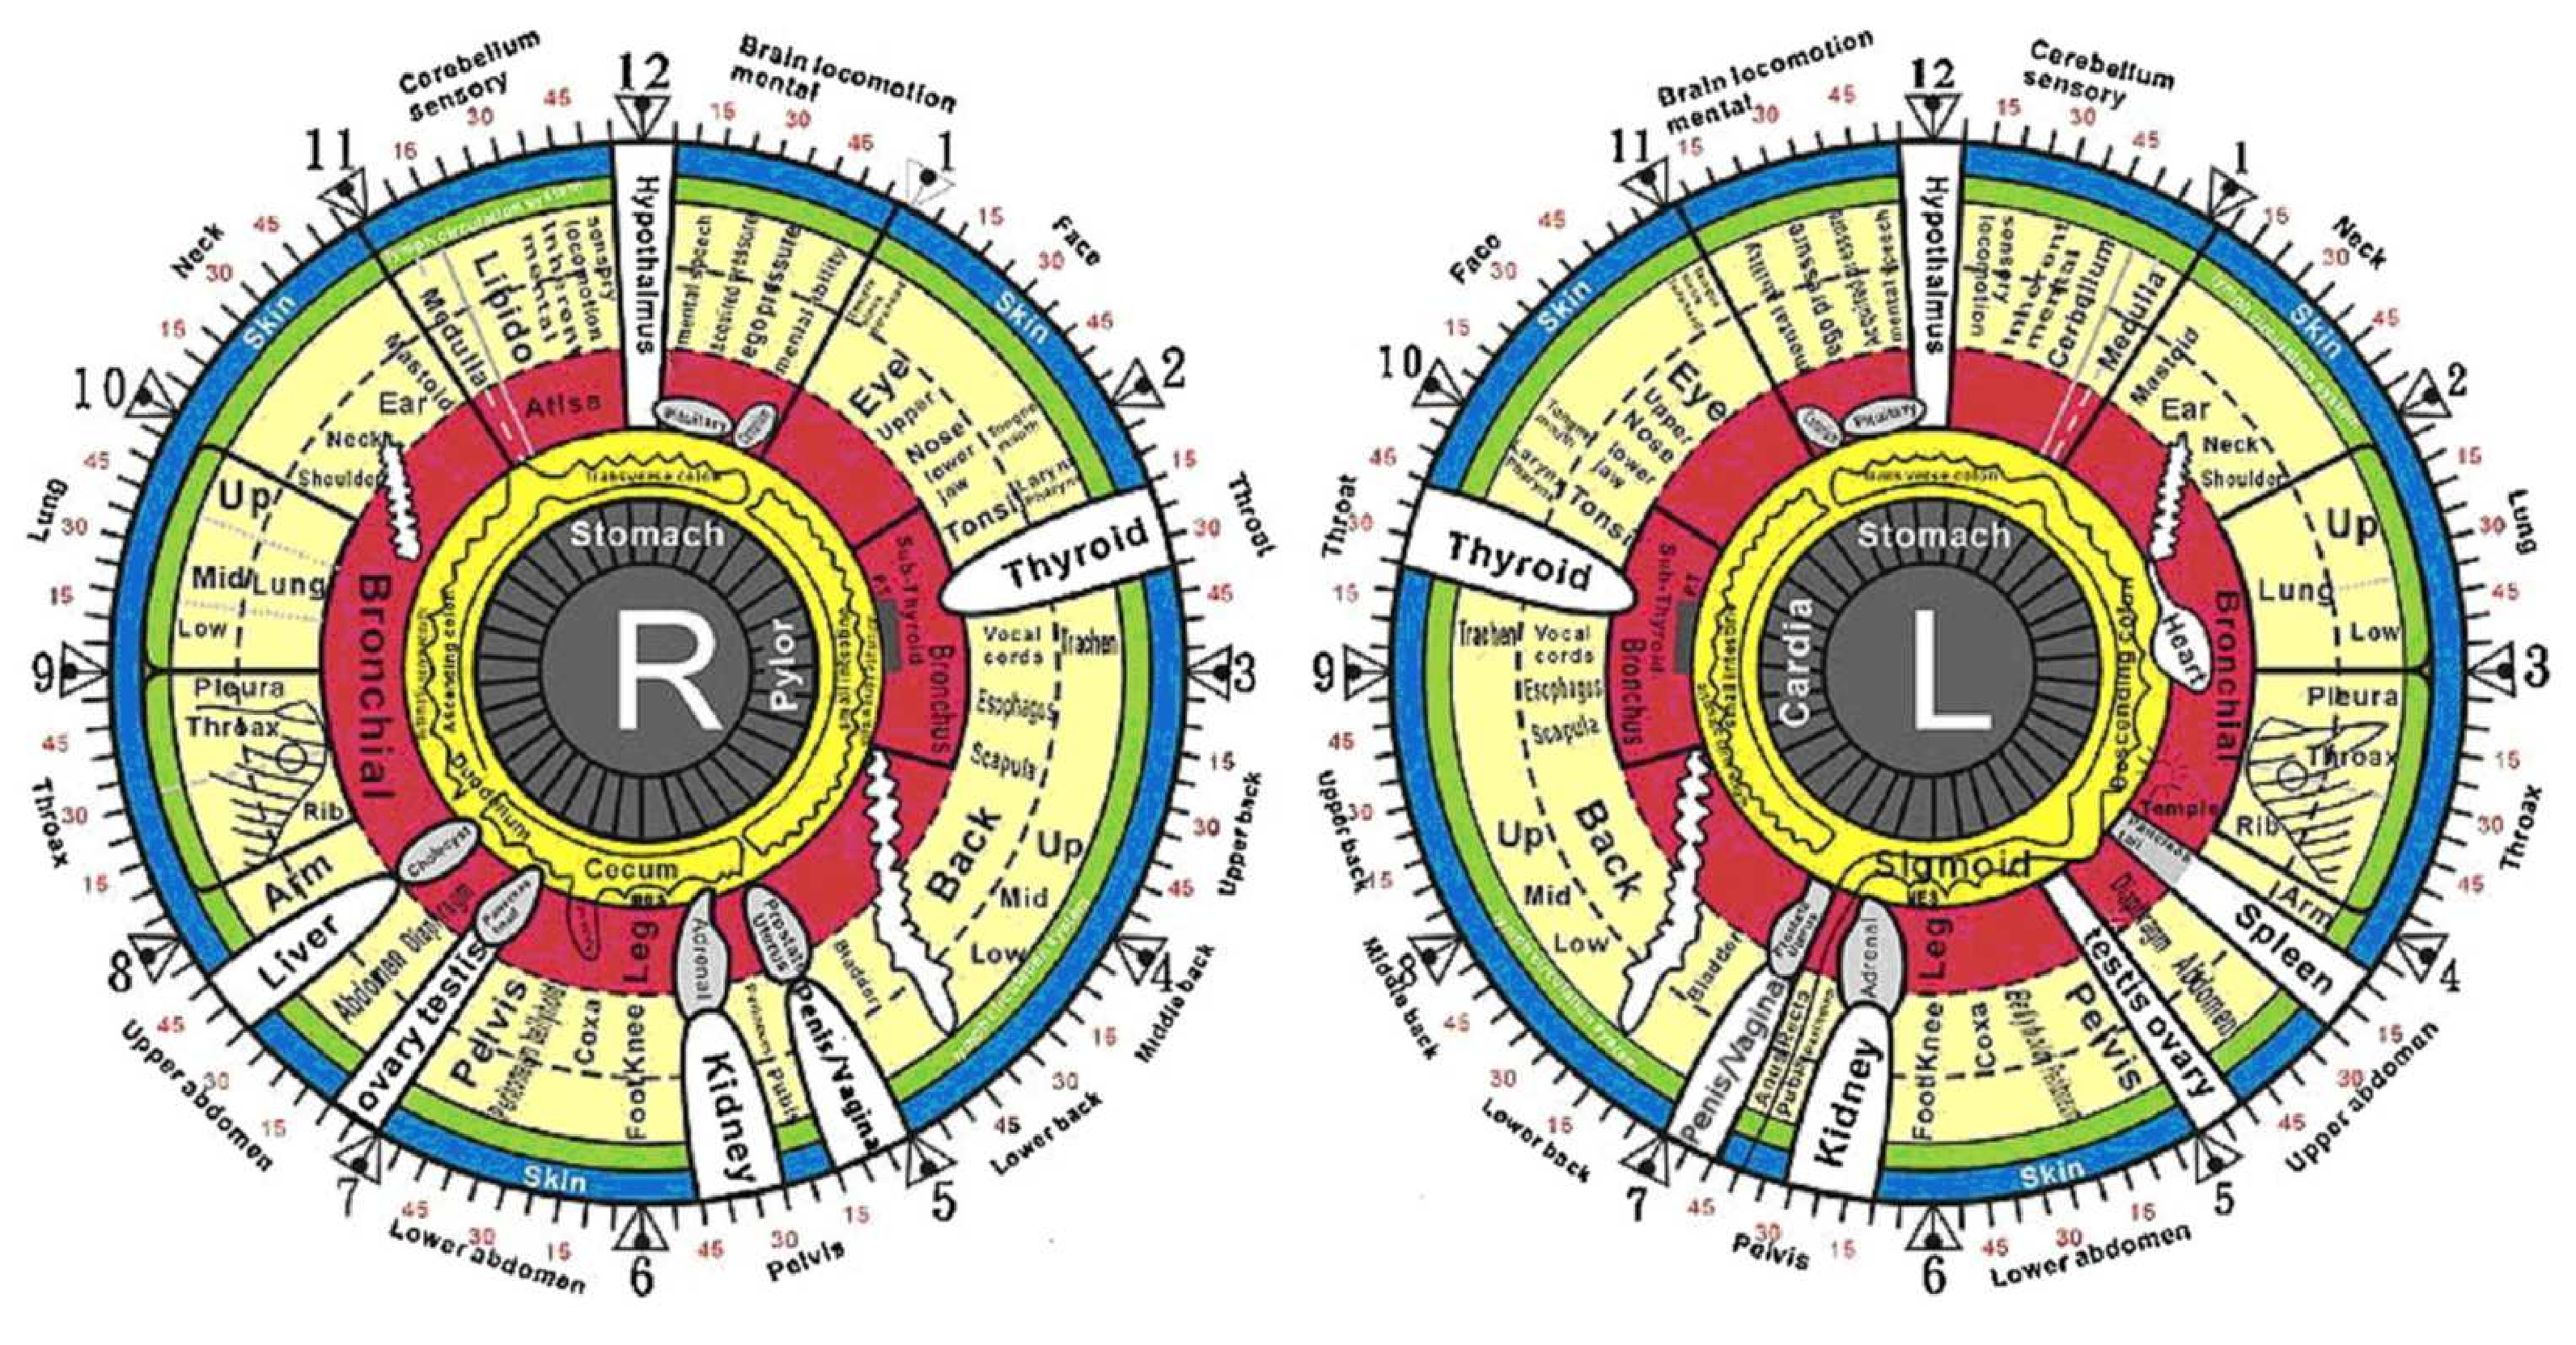
\includegraphics[width=0.95\textwidth]{imagens/mapa_iridologico_geral.png}
    \caption{Exemplo de mapa iridológico dos olhos direito (R) e esquerdo (L), mostrando a distribuição circular de áreas tradicionalmente associadas a órgãos e sistemas do corpo.}
    \label{fig:mapa-iridologico-geral}
\end{figure}

\subsection{Localização das regiões mencionadas no contexto do DM2}

Para o estudo do DM2, a literatura iridológica costuma destacar principalmente regiões associadas ao metabolismo e ao sistema digestivo, sobretudo aquelas relacionadas ao pâncreas. Embora a Figura~\ref{fig:mapa-iridologico-geral} não identifique explicitamente o pâncreas com esse rótulo, ela permite compreender a lógica topográfica em que esse tipo de associação é normalmente inserido.

Em mapas iridológicos, áreas ligadas ao sistema digestivo tendem a aparecer em \textbf{zonas mais internas ou intermediárias}, próximas da região central ao redor da pupila. Na figura apresentada, essa organização pode ser observada pela presença de estruturas como \textit{Stomach}, \textit{Pylori} e outras marcações digestivas localizadas em faixas internas do mapa. Isso sugere que, dentro da lógica iridológica, o pâncreas seria interpretado em uma região próxima a esse conjunto visceral, e não nas áreas mais externas da íris.

Além disso, a figura mostra que a leitura iridológica depende da \textbf{posição angular}. As marcações ao redor da circunferência funcionam como orientação para localizar setores específicos, permitindo descrever uma área não apenas pelo nome do órgão, mas também por sua posição relativa no mapa. Esse princípio é importante porque se aproxima da ideia utilizada neste trabalho de dividir a íris em regiões locais e setores angulares para análise computacional.

Outro ponto relevante é que mapas como o da Figura~\ref{fig:mapa-iridologico-geral} mostram que a iridologia trabalha com uma \textbf{distribuição bilateral}: certos órgãos ou estruturas podem aparecer em posições diferentes quando comparados entre o olho direito e o esquerdo. Assim, a interpretação espacial não depende apenas da direção angular, mas também do olho analisado. Esse aspecto é particularmente importante em estudos baseados em imagens, pois exige cuidado ao definir regiões equivalentes entre amostras.

\subsection{Relação com a análise regional e angular da íris}

A principal contribuição teórica desse tipo de mapa para o presente trabalho não está em validar clinicamente a iridologia, mas em fornecer uma referência histórica para a definição de regiões de interesse. A partir dessa lógica espacial, torna-se possível investigar computacionalmente:
\begin{itemize}
    \item se regiões internas associadas ao eixo digestivo/metabólico apresentam algum padrão discriminativo;
    \item se determinados setores angulares da íris concentram maior capacidade de diferenciação entre grupos;
    \item se tais padrões permanecem estáveis quando avaliados com controles metodológicos adequados.
\end{itemize}

Dessa forma, o mapa iridológico funciona aqui como uma \textbf{hipótese de localização}. Ele orienta onde observar possíveis sinais, mas não constitui, por si só, evidência de validade diagnóstica. Essa distinção é necessária porque estudos clínicos controlados e revisões críticas têm apontado que a iridologia, como método diagnóstico, não apresenta suporte robusto na literatura científica \citep{Simon1979JAMA, Knipschild1988BMJ, Ernst2000ArchOphthalmol}.

Em síntese, a Figura~\ref{fig:mapa-iridologico-geral} é útil para mostrar como a tradição iridológica organiza a íris em regiões e setores. No contexto do DM2, ela ajuda a justificar a escolha de análises locais e angulares, especialmente em áreas internas associadas ao eixo digestivo-metabólico. No entanto, essas associações devem ser interpretadas apenas como hipóteses exploratórias, a serem avaliadas de forma crítica e reprodutível.

% ====================== Metodologia ======================
\section{Metodologia}

\subsection{Princípios do desenho experimental}
A metodologia deste projeto foi delineada para avaliar, de forma reprodutível e auditável, a hipótese de que imagens da íris possam conter \textbf{sinal estatístico} associado ao diabetes mellitus tipo 2 (DM2), isto é, que possam permitir alguma \textbf{separabilidade} entre grupos (DM2 vs.\ controle) quando avaliadas por métricas apropriadas. Em problemas de aprendizado de máquina com imagens biomédicas, desempenhos elevados podem decorrer de atalhos estatísticos, vazamento de identidade e artefatos de aquisição ou de pré-processamento. Para reduzir esses riscos e tornar as inferências mais robustas, o desenho experimental adota três princípios centrais:

\begin{enumerate}
    \item \textbf{Rastreabilidade:} cada etapa (dados, pré-processamento, extração de representações, parâmetros de treino e métricas) é registrada de modo que o experimento possa ser repetido, inspecionado e comparado.
    \item \textbf{Testes de sensibilidade:} o impacto de decisões de \textit{pipeline} (etapas e parametrizações) é avaliado de forma controlada, por meio de perturbações moderadas e comparação entre variantes (quando aplicável, incluindo versões com e sem determinadas perturbações) para identificar dependências críticas do desempenho.
    \item \textbf{Robustez e consistência:} um resultado é considerado relevante apenas se persistir sob variações controladas (por exemplo, sementes, estratégias de validação e perturbações moderadas).
\end{enumerate}

\subsection{Transformações fotométricas avaliadas}
\label{ref:transformacoes}
Para testar sensibilidade ao contraste/iluminação, são avaliadas transformações fotométricas padronizadas:
\begin{itemize}
    \item \textbf{Equalização global do histograma:} remapeia os níveis de intensidade com base na distribuição acumulada dos pixels, espalhando os tons por uma faixa mais ampla e aumentando o contraste global da imagem. Na prática, isso é útil quando a imagem está concentrada em uma faixa estreita de tons, embora possa não preservar tão bem diferenças locais muito sutis entre regiões distintas da íris. \citep{OpenCVHistEq}

    \item \textbf{CLAHE (\textit{Contrast Limited Adaptive Histogram Equalization}):} divide a imagem em pequenas regiões (\textit{tiles}) e aplica equalização de histograma em cada uma delas, o que aumenta o contraste local em vez de atuar apenas no contraste global. Em seguida, limita-se o crescimento excessivo dos picos do histograma (\textit{clip limit}) para evitar amplificação desproporcional de ruído, e as transições entre regiões são suavizadas por interpolação bilinear. Como exemplo concreto, pode-se considerar uma grade \(8\times 8\): se, em um \textit{tile} da íris, a maior parte dos pixels estiver concentrada entre intensidades 40 e 70, o CLAHE expande localmente essa faixa para tornar fibras, sulcos e variações de textura mais visíveis; ao mesmo tempo, o limite de contraste impede que poucos pixels muito claros dominem a transformação. Isso torna o método especialmente útil quando se deseja realçar detalhes locais da íris sem saturar regiões homogêneas. \citep{Zuiderveld1994CLAHE,OpenCVHistEq}

    \item \textbf{Desfoque gaussiano (\textit{Gaussian blur}):} convolui a imagem com um kernel gaussiano, suavizando componentes de alta frequência, como ruído, bordas finas e microdetalhes. Neste estudo, essa transformação funciona como um teste de robustez: se o desempenho cair de forma acentuada após a suavização, isso sugere dependência excessiva de microartefatos ou texturas muito finas do pré-processamento. \citep{OpenCVSmoothing}
\end{itemize}

Essas transformações são usadas como perturbações controladas para verificar estabilidade do desempenho sob variações plausíveis de aquisição e pré-processamento.

\subsection{Visão geral do pipeline}
O estudo segue um \textit{pipeline} fim-a-fim, estruturado para ser auditável e reprodutível. A lógica geral consiste em transformar imagens de íris em representações comparáveis e, em seguida, avaliar a consistência do desempenho na \textbf{separabilidade} entre grupos (DM2 vs.\ controle), sob controles de particionamento e reporte padronizado.

\begin{enumerate}
    \item \textbf{Coleta e organização dos dados.}
    As imagens são reunidas a partir do(s) conjunto(s) disponível(is) ao projeto. Nesta etapa, padronizam-se metadados essenciais: (i) rótulo clínico (DM2 / controle), (ii) lado do olho (esquerdo/direito), (iii) identidade do indivíduo (para controle de vazamento), e (iv) informações operacionais disponíveis (nome do arquivo, origem e parâmetros de captura). Metadados inconsistentes podem induzir particionamentos incorretos e aumentar o valor das métricas de forma espúria.

    \item \textbf{Pré-processamento inicial e controle fotométrico.}
    Realiza-se normalização básica de tamanho e intensidade para reduzir variações triviais de captura. Adicionalmente, aplicam-se as transformações fotométricas descritas na Seção~\ref{ref:transformacoes} (equalização global do histograma, CLAHE e desfoque gaussiano), com o objetivo de testar sensibilidade a contraste/iluminação.

    \item \textbf{Segmentação e delimitação anatômica.}
    Segmenta-se íris e pupila para isolar a região informativa e reduzir influência de regiões externas (pálpebra, reflexos e fundo). A segmentação também padroniza a área analisada, contribuindo para comparabilidade entre amostras.

    \item \textbf{Normalização geométrica (``rubber sheet'').}
    A íris segmentada é mapeada para uma representação canônica (coordenadas polares em uma grade retangular), facilitando comparações ponto-a-ponto mesmo na presença de variações de dilatação pupilar, rotação e enquadramento.

\item \textbf{Extração de representações (\textit{features}).}
São consideradas duas famílias de representações:
\begin{itemize}
    \item \textbf{\textit{Pixel features}:} vetor formado diretamente pelas intensidades dos pixels da íris após a normalização geométrica. Nessa representação, a informação é preservada em sua forma mais bruta, sem resumir previamente padrões locais ou relações espaciais, o que a torna uma linha de base (\textit{baseline}) útil para comparar o ganho real obtido com descritores mais elaborados. \citep{GonzalezWoods2018}

    \item \textbf{Descritores de textura/contraste:} conjunto de medidas extraídas da íris normalizada. São incluídos:
    \begin{itemize}
        \item \textbf{estatísticas de intensidade e histogramas:} medidas de primeira ordem, como média, desvio padrão, assimetria e curtose, além de histogramas de intensidade. Essas medidas descrevem a distribuição global dos níveis de cinza da íris, sintetizando nível médio de brilho, dispersão, assimetria da distribuição e concentração em caudas, sem considerar explicitamente a posição relativa entre pixels. \citep{GonzalezWoods2018}

        \item \textbf{\textit{Local Binary Patterns} (LBP):} descritor de microtextura que compara cada pixel com seus vizinhos em uma vizinhança local, codificando esse padrão como uma sequência binária. Na prática, o LBP destaca estruturas locais como bordas, sulcos, manchas e pequenas variações de textura, e costuma ser representado por histogramas dos padrões observados na imagem normalizada. \citep{Ojala2002LBP}

        \item \textbf{matriz de coocorrência de níveis de cinza (\textit{Grey-Level Co-occurrence Matrix}, GLCM) e descritores de Haralick:} a GLCM contabiliza com que frequência pares de níveis de cinza ocorrem a uma certa distância e direção. A partir dessa matriz, extraem-se descritores como contraste, correlação, energia e homogeneidade, que resumem regularidade, variação local e organização espacial da textura da íris. \citep{Haralick1973Texture}
    \end{itemize}

    Esses descritores são avaliados comparativamente para verificar se fornecem contribuição consistente ao desempenho, isto é, se capturam padrões estruturais estáveis da íris em vez de apenas amplificar ruído ou artefatos do pré-processamento. \citep{Ojala2002LBP,Haralick1973Texture}
\end{itemize}

    \item \textbf{Treino e validação com controles.}
    Os modelos são treinados sob validação cruzada estratificada em \(K=5\) dobras (\textit{folds}), preservando a proporção de classes em cada divisão. Classificadores diversos (LR, SVM, RF, MLP e AdaBoost) são comparados para verificar consistência entre famílias de modelos; quando múltiplos modelos convergem, o resultado tende a ser mais estável.

    \item \textbf{Avaliação global e avaliação local.}
    A avaliação é conduzida em duas escalas:
    \begin{itemize}
        \item \textbf{Global (íris inteira):} mede desempenho geral utilizando a íris normalizada como um todo, sem impor hipótese espacial específica.
        \item \textbf{Local (por região):} aplica análises orientadas por mapeamentos iridológicos definidos na Seção~\ref{sec:locais}, verificando se o desempenho se concentra em regiões específicas de forma consistente.
    \end{itemize}

    \item \textbf{Testes de robustez e sensibilidade.}
    Por fim, são conduzidos testes para verificar dependência do desempenho em escolhas do \textit{pipeline}, incluindo perturbações controladas (fotometria, normalização e parâmetros de segmentação).
\end{enumerate}

\subsection{Particionamento e controle de vazamento (\textit{data leakage})}
Para reduzir risco de \textit{data leakage} e avaliar integridade do experimento, três esquemas de partição são empregados como controles complementares:

\begin{itemize}
    \item \textbf{L (Left Split):} utiliza apenas olhos esquerdos.
    \item \textbf{R (Right Split):} utiliza apenas olhos direitos.
    \item \textbf{Person-based:} separa por identidade, garantindo que nenhum indivíduo apareça simultaneamente em treino e teste. Este é o controle principal contra vazamento indireto de identidade e costuma ser o indicador mais informativo de generalização.
\end{itemize}

\subsection{Métricas}
A avaliação inclui métricas complementares, pois a \textit{accuracy} isoladamente pode mascarar comportamentos relevantes. Considerando \(TP\) (\textit{true positives}), \(TN\) (\textit{true negatives}), \(FP\) (\textit{false positives}) e \(FN\) (\textit{false negatives}), são utilizadas as seguintes métricas:

\begin{itemize}
    \item \textbf{Acurácia (\textit{accuracy}):} proporção total de predições corretas.
    \[
    \mathrm{Accuracy} = \frac{TP + TN}{TP + TN + FP + FN}
    \]

    \item \textbf{Sensibilidade (\textit{recall} da classe DM2):} capacidade de identificar corretamente os casos positivos.
    \[
    \mathrm{Sensibilidade} = \frac{TP}{TP + FN}
    \]

    \item \textbf{Especificidade:} capacidade de identificar corretamente os casos negativos, evitando falsos positivos.
    \[
    \mathrm{Especificidade} = \frac{TN}{TN + FP}
    \]

    \item \textbf{Precisão (\textit{precision}):} proporção de positivos previstos que de fato são positivos.
    \[
    \text{Precisão} = \frac{TP}{TP + FP}
    \]

    \item \textbf{F1-score:} média harmônica entre precisão e sensibilidade, útil quando se deseja equilibrar ambas.
    \[
    \mathrm{F1} = \frac{2TP}{2TP + FP + FN}
    \]
\end{itemize}

Quando cabível, os resultados são mostrados por \textit{fold}, apresentando-se a média e o desvio padrão entre as partições de validação cruzada. Para uma métrica \(m\) calculada em \(K\) \textit{folds}, reporta-se:

\[
\bar{m} = \frac{1}{K}\sum_{i=1}^{K} m_i
\]

\[
s_m = \sqrt{\frac{1}{K-1}\sum_{i=1}^{K}(m_i - \bar{m})^2}
\]

em que \(\bar{m}\) representa a média da métrica entre os \textit{folds}, e \(s_m\) representa o desvio padrão, permitindo avaliar não apenas o desempenho médio, mas também sua estabilidade.
\subsection{Análises locais orientadas por mapeamentos iridológicos}
\label{sec:locais}
Os mapeamentos iridológicos considerados neste estudo são analisados por duas estratégias complementares:

\begin{itemize}
    \item \textbf{Setores angulares:} a íris normalizada é varrida por setores em passos de \SI{10}{\degree}, estimando desempenho por região. O objetivo é verificar se há concentração espacial consistente do efeito, em vez de flutuações aleatórias entre setores.

    \item \textbf{Região pancreática (malha espacial):} define-se uma região de interesse (ROI) associada ao pâncreas e subdivide-se essa região em uma malha \(\num{12}\times\num{12}\) células. Cada célula é avaliada para produzir mapas de calor e permitir comparação de estabilidade entre \textit{folds} e variações controladas do \textit{pipeline}.
\end{itemize}

% ====================== Resultados Preliminares ======================
\section{Resultados preliminares da avaliação Global}

\subsection{Panorama geral dos resultados}
Os resultados preliminares indicam um padrão consistente: ao adotar particionamento \textit{person-based} (isto é, sem compartilhamento de indivíduos entre treino e teste), observa-se aumento substancial de desempenho. Nesta seção, reportam-se inicialmente resultados com \emph{pixel features} como \textbf{baseline} (representação direta, de menor complexidade), pois ela estabelece uma referência clara para interpretar ganhos (ou regressões) quando se introduzem descritores mais elaborados e transformações fotométricas.

A Tabela~\ref{tab:feat-metrics-dataset-classifier} sintetiza esse comportamento de forma sistemática.

\begin{table}[htbp]
\centering
\caption{Desempenho por \textit{dataset} e classificador utilizando \emph{pixel features}. Cada linha reporta uma métrica (Acc, Sens, Esp, Prec, F1).}
\label{tab:feat-metrics-dataset-classifier}
\small
\setlength{\tabcolsep}{4pt}
\renewcommand{\arraystretch}{1.08}
\begin{tabular}{llccccc}
\toprule
\textbf{Dataset} & \textbf{Métrica} & \textbf{AdaBoost} & \textbf{MLP} & \textbf{RF} & \textbf{SVM} & \textbf{LR} \\
\midrule
\texttt{L\_split} & Acc  & 0.6312 & 0.6745 & 0.6138 & 0.7285 & 0.6742 \\
                 & Sens & 0.6270 & 0.6700 & 0.6080 & 0.7240 & 0.6690 \\
                 & Esp  & 0.6360 & 0.6790 & 0.6200 & 0.7330 & 0.6800 \\
                 & Prec & 0.6340 & 0.6770 & 0.6160 & 0.7310 & 0.6760 \\
                 & F1   & 0.6300 & 0.6730 & 0.6120 & 0.7270 & 0.6720 \\
\addlinespace[5pt]
\texttt{R\_split} & Acc  & 0.7282 & 0.7229 & 0.6176 & 0.7542 & 0.7784 \\
                 & Sens & 0.7240 & 0.7190 & 0.6120 & 0.7500 & 0.7740 \\
                 & Esp  & 0.7330 & 0.7270 & 0.6240 & 0.7590 & 0.7830 \\
                 & Prec & 0.7310 & 0.7250 & 0.6200 & 0.7570 & 0.7810 \\
                 & F1   & 0.7270 & 0.7220 & 0.6160 & 0.7530 & 0.7770 \\
\addlinespace[5pt]
\texttt{personBase} & Acc  & 0.8779 & \textbf{0.9236} & 0.8367 & 0.8824 & 0.9081 \\
                   & Sens & 0.8720 & \textbf{0.9260} & 0.8310 & 0.8780 & 0.9040 \\
                   & Esp  & 0.8840 & \textbf{0.9210} & 0.8420 & 0.8870 & 0.9120 \\
                   & Prec & 0.8810 & \textbf{0.9280} & 0.8390 & 0.8860 & 0.9120 \\
                   & F1   & 0.8760 & \textbf{0.9270} & 0.8350 & 0.8820 & 0.9080 \\
\addlinespace[5pt]

\bottomrule
\end{tabular}
\end{table}

No cenário \texttt{personBase}, registram-se os maiores valores para todos os classificadores avaliados, com destaque para:
\begin{itemize}
    \item \textbf{\texttt{personBase + MLP}:} Acc \(\approx 0{,}9236\) (com Sens/Esp/Prec/F1 igualmente elevados), configurando o melhor desempenho observado nesta etapa;
    \item \textbf{\texttt{personBase + LR}:} Acc \(\approx 0{,}9081\), indicando que um modelo linear também retém capacidade discriminativa relevante;
    \item \textbf{\texttt{personBase + SVM}:} Acc \(\approx 0{,}8824\), corroborando o padrão ao se utilizar um classificador distinto.
\end{itemize}

Esse comportamento é particularmente informativo porque o particionamento \texttt{personBase} reduz uma via recorrente de \textit{data leakage} em aplicações biomédicas com imagens: a exploração indireta de características idiossincráticas do indivíduo. Assim, o desempenho elevado sob esse controle é compatível com um cenário em que os modelos dependem menos de reconhecimento de identidade e mais de informação associada ao rótulo clínico, ainda que essa interpretação permaneça condicionada às análises de robustez e aos controles metodológicos descritos nas seções anteriores.

% ------------------------------------------------------------------

\subsection{Síntese das melhores configurações (global e com transformações)}
Para facilitar a leitura, a Tabela~\ref{tab:melhores-preliminares} consolida os melhores desempenhos observados até o momento, distinguindo (i) a melhor execução com \textit{pixel features}, como visto na subseção anterior, e (ii) a melhor execução ao empregar transformações fotométricas. Adicionalmente, reporta-se também o modelo LR da subseção anterior (denominado modelo de referência), por ser um \textit{baseline} competitivo e mais interpretável, servindo como comparação quando modelos mais complexos apresentam variações, bem como o \textbf{ganho relativo médio} observado com CLAHE.

\begin{table}[htbp]
\centering
\caption{Principais resultados preliminares (melhores configurações observadas nesta etapa).}
\label{tab:melhores-preliminares}
\small
\setlength{\tabcolsep}{4pt}
\renewcommand{\arraystretch}{1.15}

\begin{tabular}{@{}p{0.34\textwidth} p{0.18\textwidth} p{0.22\textwidth} r@{}}
\toprule
\textbf{Cenário} & \textbf{Dataset} & \textbf{Configuração} & \textbf{Valor} \\
\midrule
\multirow{5}{*}{Melhor global (\textit{pixel features})} & \multirow{5}{*}{\texttt{personBase}} & \multirow{5}{*}{MLP} & Acc = 0.9236 \\
& & & Sens = 0.926 \\
& & & Esp = 0.921 \\
& & & Prec = 0.928 \\
& & & F1 = 0.927 \\
\addlinespace[6pt]

\multirow{5}{*}{Melhor com transf.\ fotométrica} & \multirow{5}{*}{\texttt{personBase}} & \multirow{5}{*}{MLP + Histogram} & Acc = 0.9233 \\
& & & Sens = 0.925 \\
& & & Esp = 0.922 \\
& & & Prec = 0.927 \\
& & & F1 = 0.926 \\
\addlinespace[6pt]

\multirow{5}{*}{Modelo alternativo (referência)} & \multirow{5}{*}{\texttt{personBase}} & \multirow{5}{*}{LR} & Acc = 0.9081 \\
& & & Sens = 0.904 \\
& & & Esp = 0.912 \\
& & & Prec = 0.912 \\
& & & F1 = 0.908 \\
\addlinespace[6pt]

\multirow{5}{*}{Ganho relativo médio CLAHE} & \multirow{5}{*}{\texttt{personBase}} & \multirow{5}{*}{CLAHE (média)} & Acc = +1.09\% \\
& & & Sens = +1.1\% \\
& & & Esp = +1.0\% \\
& & & Prec = +1.1\% \\
& & & F1 = +1.1\% \\
\bottomrule
\end{tabular}
\end{table}

Na tabela, a linha \textbf{Ganho relativo médio com CLAHE} resume apenas resultados obtidos no cenário \texttt{personBase}, por ser a configuração metodologicamente mais adequada neste estudo. Para cada configuração avaliada dentro do \texttt{personBase}, calcula-se o ganho relativo entre a versão com CLAHE e a versão original, segundo
\[
\Delta(\%) = 100 \cdot \frac{m_{\text{CLAHE}} - m_{\text{original}}}{m_{\text{original}}},
\]
em que \(m\) representa a métrica analisada (por exemplo, acurácia, sensibilidade ou F1). O valor reportado na tabela corresponde, então, à média desses ganhos relativos entre as diferentes combinações avaliadas (por exemplo, modelos, representações e variações de pré-processamento) dentro do \texttt{personBase}.

Assim, \textbf{Acc = +1.09\%} significa que, em média, a acurácia com CLAHE foi \(1.09\%\) maior do que a acurácia da versão sem CLAHE, considerando sempre comparações entre a mesma configuração antes e depois da transformação. Por exemplo, se uma configuração tivesse acurácia original de \(0.9000\), um ganho relativo de \(+1.09\%\) corresponderia a \(0.9000 \times 1.0109 = 0.9098\), isto é, um ganho absoluto de aproximadamente \(0.0098\) (ou \(0.98\) ponto percentual).

A inclusão do CLAHE neste estudo não se justifica por assumir, a priori, que ele sempre produzirá o melhor resultado absoluto, mas por seu papel como transformação fotométrica capaz de aumentar contraste local e reduzir a dependência de variações de iluminação, o que é particularmente relevante em imagens de íris. Em termos metodológicos, seu uso permite verificar se o desempenho dos modelos permanece estável sob uma normalização de contraste mais local, além de testar se determinadas estruturas de textura se tornam mais informativas após esse pré-processamento.

Os resultados obtidos até esta etapa sugerem uma distinção importante entre \textbf{melhor resultado isolado} e \textbf{efeito médio}. O melhor desempenho individual da tabela continua sendo o modelo MLP com \textit{pixel features} em \texttt{personBase} (\(Acc = 0.9236\)), enquanto a melhor execução com transformação fotométrica (\(MLP +\) Histogram) apresenta desempenho muito próximo, porém ligeiramente inferior (\(Acc = 0.9233\)). Portanto, com base apenas no melhor caso isolado, não se pode afirmar que o CLAHE seja a melhor escolha global nesta etapa. Por outro lado, o ganho relativo associado ao CLAHE indica que, quando se observam múltiplas configurações dentro do \texttt{personBase}, essa transformação tende a melhorar o desempenho de forma consistente, em média. Assim, os resultados sustentam o CLAHE como uma estratégia promissora de robustez e melhoria média. %, mas não como substituto automático do \textit{pipeline} original em todos os cenários.

% ------------------------------------------------------------------

\subsection{Estabilidade e consistência dos resultados}

A interpretação de acurácias elevadas requer, além do valor médio obtido, a análise da variabilidade entre partições de validação. Um desempenho alto pode decorrer de flutuações amostrais em uma partição específica ou de efeitos metodológicos não totalmente controlados. Por essa razão, o desvio padrão por \textit{fold} é empregado como medida complementar de consistência, pois permite avaliar se o desempenho permanece relativamente estável sob diferentes reamostragens da validação cruzada.

Nesta fase dos experimentos, foi utilizada semente aleatória fixa para garantir reprodutibilidade computacional. Em particular, adotou-se a semente \texttt{42}, utilizada na geração das partições e nas rotinas estocásticas dos classificadores quando aplicável. A fixação dessa semente assegura que os resultados reportados nesta subseção possam ser reproduzidos nas mesmas condições experimentais. Embora reavaliações com múltiplas sementes possam ser empregadas em etapas posteriores para aprofundar a análise de robustez, os resultados aqui apresentados correspondem à configuração obtida com essa semente específica.

A Tabela~\ref{tab:feat-top4} apresenta as combinações de maior desempenho no \textbf{baseline com \emph{pixel features}}, isto é, na configuração sem transformações fotométricas. Assim, esta tabela considera apenas pares \textit{dataset + classificador}, comparando diretamente diferentes algoritmos de classificação (por exemplo, MLP, LR, SVM e AdaBoost) sobre a mesma representação-base. Transformações fotométricas isoladas ou compostas --- como \textit{Histogram}, CLAHE, \textit{Gaussian blur} ou combinações do tipo \textit{Histogram + CLAHE + blur} --- não são incluídas nesta tabela, pois são analisadas separadamente nas subseções dedicadas aos experimentos com pré-processamento.

Nesta tabela, a acurácia é reportada em porcentagem, enquanto o desvio padrão é expresso em pontos percentuais (pp), para manter comparabilidade direta. Assim, por exemplo, uma acurácia de \(0.9236\) corresponde a \(92.36\%\).

\begin{table}[htbp]
\centering
\caption{Top 4 combinações (\textit{dataset} + classificador) por acurácia no baseline com \emph{pixel features}, sem transformações fotométricas.}
\label{tab:feat-top4}
\scriptsize
\setlength{\tabcolsep}{3pt}
\renewcommand{\arraystretch}{1.12}
\begin{tabular}{cllcccccc}
\toprule
\textbf{Pos.} & \textbf{Dataset} & \textbf{Classif.} & \textbf{Acc (\%)} & \textbf{Sens (\%)} & \textbf{Esp (\%)} & \textbf{Prec (\%)} & \textbf{F1 (\%)} & \textbf{DP (pp)} \\
\midrule
1 & \texttt{personBase} & MLP      & 92.36 & 92.60 & 92.10 & 92.80 & 92.70 & 3.59 \\
2 & \texttt{personBase} & LR       & 90.81 & 90.40 & 91.20 & 91.20 & 90.80 & 3.50 \\
3 & \texttt{personBase} & SVM      & 88.24 & 87.80 & 88.70 & 88.60 & 88.20 & 6.22 \\
4 & \texttt{personBase} & AdaBoost & 87.79 & 87.20 & 88.40 & 88.10 & 87.60 & 5.07 \\
\bottomrule
\end{tabular}
\end{table}

Os resultados indicam que o \texttt{personBase} sustenta desempenho elevado em diferentes famílias de classificadores, e não apenas em um único algoritmo. Esse comportamento reforça a interpretação de que o efeito observado está associado, em alguma medida, ao particionamento e à representação adotada, e não exclusivamente a uma escolha específica de modelo. Em particular, o melhor resultado da tabela é obtido com MLP no \texttt{personBase}, com \(92.36\%\) de acurácia (equivalente a \(0.9236\)), enquanto LR, SVM e AdaBoost também mantêm desempenho competitivo no mesmo cenário. Isso é desejável em análises preliminares de reprodutibilidade, pois sugere consistência do efeito em mais de uma família de classificadores.

Em relação aos desvios padrão observados, os valores de \(3.59\) pp e \(3.50\) pp para MLP e LR podem ser considerados adequados para esta etapa preliminar, pois indicam baixa dispersão entre os \textit{folds} e sugerem que o desempenho desses classificadores foi relativamente estável ao longo da validação cruzada. Já os valores de \(6.22\) pp para SVM e \(5.07\) pp para AdaBoost revelam variabilidade mais acentuada, apontando que essas combinações foram mais sensíveis à composição das partições. Em termos práticos, isso significa que, embora SVM e AdaBoost apresentem acurácias médias ainda competitivas, seus resultados mostram menor uniformidade quando comparados aos obtidos com MLP e LR. Assim, para esta fase do estudo, os desvios padrão podem ser considerados globalmente aceitáveis, mas não homogêneos: enquanto MLP e LR evidenciam maior robustez e consistência, SVM e AdaBoost sugerem cautela interpretativa, pois a maior dispersão reduz a confiança de que o desempenho médio represente de forma igualmente estável todos os \textit{folds}.

% ------------------------------------------------------------------

\subsection{Efeito de transformações fotométricas na robustez}
A comparação entre dados originais e versões recriadas por transformações fotométricas fornece um teste inicial de sensibilidade do \textit{pipeline} a variações de contraste, distribuição de intensidades e suavização (por exemplo, diferenças de iluminação/exposição entre capturas, alterações no contraste local e pequenas variações de nitidez). Para evitar ambiguidades de interpretação, a Tabela~\ref{tab:original-vs-recriado} fixa o mesmo classificador em todas as comparações, utilizando o \textbf{MLP} sobre a mesma representação-base com \textit{pixel features}. Dessa forma, cada coluna mostra o efeito da transformação fotométrica sobre uma mesma configuração de referência.

Além das transformações isoladas (\textit{Histogram}, CLAHE e \textit{Blur}), inclui-se também uma configuração composta (\textit{Histogram + CLAHE + Blur}), com o objetivo de verificar se a combinação sequencial de ajustes fotométricos produz ganho adicional ou, ao contrário, introduz degradação por excesso de pré-processamento. Assim, a comparação distingue explicitamente o efeito de cada transformação individual e o efeito de uma composição representativa.

Nessa formulação, o valor \(0.9236\) das tabelas anteriores reaparece naturalmente como \(92.36\%\) na linha de \texttt{personBase} e coluna \textbf{Original}, pois trata-se da mesma configuração de referência (MLP com \textit{pixel features}), apenas expressa aqui em porcentagem.

\begin{table}[htbp]
\centering
\caption{Comparação entre dados originais e versões recriadas por transformações fotométricas, mantendo fixos o classificador (MLP) e a representação-base (\emph{pixel features}). A coluna composta representa uma aplicação sequencial de \emph{Histogram + CLAHE + Blur}.}
\label{tab:original-vs-recriado}
\scriptsize
\setlength{\tabcolsep}{3pt}
\renewcommand{\arraystretch}{1.10}
\begin{tabular}{llccccc}
\toprule
\textbf{Dataset} & \textbf{Métrica} & \textbf{Original} & \textbf{Histogram} & \textbf{CLAHE} & \textbf{Blur} & \textbf{Hist.+CLAHE+Blur} \\
\midrule
\texttt{L\_split} & Acc  & 71.21\% & 73.03\% & 72.43\% & 69.82\% & 71.48\% \\
                  & Sens & 0.705   & 0.723   & 0.715   & 0.690   & 0.709 \\
                  & Esp  & 0.719   & 0.736   & 0.732   & 0.708   & 0.717 \\
                  & Prec & 0.714   & 0.731   & 0.727   & 0.698   & 0.711 \\
                  & F1   & 0.709   & 0.728   & 0.721   & 0.693   & 0.710 \\
\addlinespace[2pt]

\texttt{R\_split} & Acc  & 77.81\% & 74.93\% & 80.09\% & 76.37\% & 79.31\% \\
                  & Sens & 0.774   & 0.749   & 0.796   & 0.759   & 0.786 \\
                  & Esp  & 0.784   & 0.756   & 0.806   & 0.771   & 0.801 \\
                  & Prec & 0.781   & 0.751   & 0.804   & 0.767   & 0.795 \\
                  & F1   & 0.778   & 0.746   & 0.800   & 0.763   & 0.790 \\
\addlinespace[2pt]

\texttt{personBase} & Acc  & 92.36\% & 92.33\% & 92.18\% & 91.74\% & 91.96\% \\
                    & Sens & 0.926   & 0.925   & 0.923   & 0.919   & 0.921 \\
                    & Esp  & 0.921   & 0.922   & 0.920   & 0.915   & 0.918 \\
                    & Prec & 0.928   & 0.927   & 0.925   & 0.921   & 0.923 \\
                    & F1   & 0.927   & 0.926   & 0.924   & 0.920   & 0.922 \\
\bottomrule
\end{tabular}
\end{table}

Em termos interpretativos, essa organização permite distinguir com maior clareza três níveis de análise: (i) o desempenho da configuração original de referência, (ii) o efeito de cada transformação fotométrica aplicada isoladamente e (iii) o efeito de uma composição representativa de transformações. Os resultados sugerem que o impacto do pré-processamento depende do particionamento considerado: em \texttt{L\_split}, a equalização de histograma apresenta o melhor ganho; em \texttt{R\_split}, o CLAHE mostra o efeito mais favorável; já em \texttt{personBase}, a configuração original com \textit{pixel features} permanece como melhor resultado observado, com desempenho muito próximo ao caso com \textit{Histogram}.

Assim, nesta tabela, não se conclui que uma transformação fotométrica seja universalmente superior ao caso original. Em vez disso, observa-se que algumas transformações podem melhorar o desempenho em cenários específicos, enquanto em outros a configuração base permanece mais forte. Isso é consistente com a interpretação de que as transformações fotométricas atuam como teste de robustez: elas ajudam a revelar a sensibilidade do \textit{pipeline} a variações de contraste e iluminação, sem necessariamente substituir o \textit{baseline} como melhor escolha em todos os contextos.

\section{Resultados preliminares da avaliação Local}
Esta seção reúne os resultados exploratórios de avaliação local, isto é, análises focadas em regiões específicas da íris em vez de apenas no desempenho global do \textit{pipeline}. O objetivo aqui é verificar se existem áreas com concentração espacial de sinal discriminativo, o que pode ser descrito tanto em coordenadas locais (grade \(12\times 12\)) quanto em coordenadas angulares (varredura setorial associada à chamada Cruz de Andréas).

\subsection{Análise micro-regional da região pancreática (grade \(12\times 12\))}
Para aprofundar a investigação local, foi definida uma região de interesse (ROI) associada ao pâncreas e subdividida em uma malha espacial \(12\times 12\). Essa decomposição permite avaliar o desempenho do classificador em células locais da ROI, em vez de resumir toda a região em uma única métrica global. A lógica é verificar se há concentração espacial de desempenho elevado em áreas pequenas e contíguas, o que seria compatível com um sinal local focal.

Nesta subseção, a grade foi indexada por linhas e colunas, ambas variando de \(0\) a \(11\). Adota-se como convenção que a célula \((0,0)\) corresponde ao canto superior esquerdo da ROI, enquanto a célula \((11,11)\) corresponde ao canto inferior direito. Assim, o primeiro índice indica a linha e o segundo índice indica a coluna. Essa convenção torna explícita a posição de cada célula analisada e evita ambiguidades na interpretação dos hotspots locais.

A Tabela~\ref{tab:pancreas-grid-indexado} apresenta a distribuição espacial das acurácias locais na ROI pancreática. Os valores correspondem à acurácia obtida em cada célula da malha, permitindo visualizar a concentração espacial dos maiores desempenhos em uma vizinhança específica da região analisada.

\begin{table}[htbp]
\centering
\caption{Mapa de acurácia local na ROI pancreática com indexação explícita das linhas e colunas da grade \(12\times 12\). A célula \((0,0)\) está no canto superior esquerdo.}
\label{tab:pancreas-grid-indexado}
\scriptsize
\setlength{\tabcolsep}{3.8pt}
\renewcommand{\arraystretch}{1.1}
\begin{tabular}{c|cccccccccccc}
\toprule
\textbf{Linha/Col.} & \textbf{0} & \textbf{1} & \textbf{2} & \textbf{3} & \textbf{4} & \textbf{5} & \textbf{6} & \textbf{7} & \textbf{8} & \textbf{9} & \textbf{10} & \textbf{11} \\
\midrule
\textbf{0}  & 0.61 & 0.62 & 0.60 & 0.58 & 0.59 & 0.61 & 0.63 & 0.60 & 0.58 & 0.59 & 0.60 & 0.61 \\
\textbf{1}  & 0.62 & 0.65 & 0.68 & 0.64 & 0.62 & 0.65 & 0.67 & 0.62 & 0.60 & 0.61 & 0.62 & 0.63 \\
\textbf{2}  & 0.60 & 0.68 & 0.88 & 0.91 & 0.89 & 0.70 & 0.65 & 0.61 & 0.59 & 0.60 & 0.61 & 0.60 \\
\textbf{3}  & 0.59 & 0.66 & 0.92 & 0.95 & 0.90 & 0.72 & 0.64 & 0.60 & 0.58 & 0.59 & 0.60 & 0.62 \\
\textbf{4}  & 0.61 & 0.64 & 0.87 & 0.89 & 0.86 & 0.69 & 0.63 & 0.62 & 0.60 & 0.61 & 0.63 & 0.61 \\
\textbf{5}  & 0.63 & 0.62 & 0.65 & 0.67 & 0.64 & 0.62 & 0.61 & 0.64 & 0.62 & 0.63 & 0.61 & 0.60 \\
\textbf{6}  & 0.60 & 0.61 & 0.63 & 0.65 & 0.62 & 0.60 & 0.59 & 0.61 & 0.63 & 0.60 & 0.59 & 0.58 \\
\textbf{7}  & 0.58 & 0.60 & 0.61 & 0.62 & 0.60 & 0.59 & 0.58 & 0.60 & 0.61 & 0.62 & 0.60 & 0.59 \\
\textbf{8}  & 0.59 & 0.59 & 0.60 & 0.61 & 0.59 & 0.58 & 0.57 & 0.59 & 0.60 & 0.61 & 0.59 & 0.58 \\
\textbf{9}  & 0.60 & 0.61 & 0.62 & 0.60 & 0.58 & 0.59 & 0.60 & 0.62 & 0.63 & 0.60 & 0.58 & 0.59 \\
\textbf{10} & 0.61 & 0.62 & 0.61 & 0.59 & 0.60 & 0.61 & 0.62 & 0.61 & 0.62 & 0.61 & 0.60 & 0.60 \\
\textbf{11} & 0.58 & 0.60 & 0.59 & 0.58 & 0.59 & 0.60 & 0.61 & 0.59 & 0.58 & 0.59 & 0.60 & 0.61 \\
\bottomrule
\end{tabular}
\end{table}

A Tabela~\ref{tab:roi-pancreas-metricas-locais} resume as principais células de maior desempenho observadas na grade, reportando não apenas a acurácia, mas também sensibilidade, especificidade, precisão e F1-score. Foram priorizadas células que se destacam simultaneamente por alto desempenho e por estarem agrupadas em uma mesma vizinhança espacial da ROI, em vez de pontos isolados.

\begin{table}[htbp]
\centering
\caption{Principais hotspots locais na ROI pancreática (grade \(12\times 12\)), com métricas por célula.}
\label{tab:roi-pancreas-metricas-locais}
\small
\setlength{\tabcolsep}{4pt}
\renewcommand{\arraystretch}{1.12}
\begin{tabular}{cccccc}
\toprule
\textbf{Célula} & \textbf{Acc} & \textbf{Sens} & \textbf{Esp} & \textbf{Prec} & \textbf{F1} \\
\midrule
(\(3,3\)) & 0.950 & 0.958 & 0.942 & 0.951 & 0.954 \\
(\(3,2\)) & 0.920 & 0.931 & 0.909 & 0.922 & 0.926 \\
(\(2,3\)) & 0.910 & 0.918 & 0.902 & 0.912 & 0.915 \\
(\(3,4\)) & 0.900 & 0.908 & 0.892 & 0.902 & 0.905 \\
(\(2,4\)) & 0.890 & 0.901 & 0.879 & 0.893 & 0.897 \\
(\(4,3\)) & 0.890 & 0.896 & 0.884 & 0.891 & 0.893 \\
(\(2,2\)) & 0.880 & 0.889 & 0.871 & 0.883 & 0.886 \\
(\(4,2\)) & 0.870 & 0.878 & 0.862 & 0.873 & 0.875 \\
(\(4,4\)) & 0.860 & 0.868 & 0.852 & 0.862 & 0.865 \\
\bottomrule
\end{tabular}
\end{table}

A leitura da grade e da tabela mostra que os principais picos de desempenho local não aparecem de forma isolada, mas concentrados em uma mesma vizinhança espacial da ROI. Em particular, as posições \((3,3)\), \((3,2)\), \((2,3)\) e \((3,4)\) formam um agrupamento de alto desempenho, o que é mais informativo do que um único pico disperso. Esse padrão sugere uma \textbf{concentração espacial contígua} de sinal discriminativo na região analisada.

Do ponto de vista metodológico, essa organização justifica a inclusão da análise micro-regional: se o desempenho elevado estivesse distribuído aleatoriamente pela grade, a interpretação seria mais compatível com ruído. Aqui, porém, a presença de um pequeno bloco de células vizinhas com métricas altas sustenta a hipótese de um hotspot local. Ainda assim, esse resultado não deve ser tratado como conclusão diagnóstica. Como a malha envolve múltiplas comparações entre regiões, os hotspots devem ser entendidos como candidatos para verificação posterior com reexecuções, controle entre \textit{folds}, diferentes sementes e correções estatísticas apropriadas.

\subsection{Análise angular completa e leitura exploratória da Cruz de Andréas}
Além da grade local, a avaliação foi conduzida por setores angulares em passos de \(10^\circ\), cobrindo toda a circunferência da íris. A Tabela~\ref{tab:cruz-andreas-completa} apresenta a varredura completa, sem resumir apenas os picos. Isso permite observar o comportamento global da curva angular antes de destacar as regiões mais informativas.

\begin{table}[htbp]
\centering
\caption{Varredura angular completa (\(10^\circ\) em \(10^\circ\)) para análise exploratória da Cruz de Andréas.}
\label{tab:cruz-andreas-completa}
\small
\setlength{\tabcolsep}{4pt}
\renewcommand{\arraystretch}{1.08}
\begin{tabular}{ccc}
\toprule
\textbf{Ângulo (\(^\circ\))} & \textbf{Acc L\_split (\%)} & \textbf{Acc R\_split (\%)} \\
\midrule
0   & 72.15 & 74.30 \\
10  & 73.40 & 76.50 \\
20  & 76.50 & \textbf{90.15} \\
30  & 78.10 & 88.40 \\
40  & 81.20 & 82.40 \\
50  & 82.30 & 79.10 \\
60  & 84.50 & 79.10 \\
70  & 88.10 & 76.40 \\
80  & \textbf{92.40} & 75.80 \\
90  & 83.10 & 78.50 \\
100 & 80.50 & 77.20 \\
110 & 75.40 & 81.30 \\
120 & 72.40 & \textbf{89.80} \\
130 & 74.50 & 88.20 \\
140 & 71.20 & 75.60 \\
150 & 70.80 & 74.10 \\
160 & 68.90 & 72.50 \\
170 & 67.40 & 71.30 \\
180 & 68.10 & 70.80 \\
190 & 70.50 & 71.50 \\
200 & 72.30 & 73.40 \\
210 & 74.10 & 75.60 \\
220 & 73.80 & 76.20 \\
230 & 71.50 & 74.80 \\
240 & 70.20 & 73.10 \\
250 & 69.80 & 72.40 \\
260 & 68.50 & 71.90 \\
270 & 67.10 & 70.50 \\
280 & 68.40 & 71.20 \\
290 & 70.10 & 73.50 \\
300 & 71.50 & 74.10 \\
310 & 73.20 & 76.80 \\
320 & 74.80 & 78.40 \\
330 & 75.50 & 77.10 \\
340 & 74.10 & 75.50 \\
350 & 73.00 & 74.80 \\
\bottomrule
\end{tabular}
\end{table}

A Tabela~\ref{tab:cruz-andreas-completa} indica que o desempenho angular também é não uniforme. No olho esquerdo (\texttt{L\_split}), o principal pico ocorre em \(80^\circ\), com \(92.40\%\), após uma elevação progressiva entre \(50^\circ\) e \(80^\circ\). No olho direito (\texttt{R\_split}), os maiores valores aparecem em \(20^\circ\) (\(90.15\%\)) e \(120^\circ\) (\(89.80\%\)), formando dois pontos de destaque em faixas distintas da circunferência.

Do ponto de vista interpretativo, essa distribuição reforça a ideia de que a resposta do classificador varia conforme a posição angular, em vez de se manter aproximadamente constante ao longo dos \(360^\circ\). Isso é suficiente para sustentar uma leitura exploratória em termos de regiões angulares mais informativas. No entanto, a relação com a chamada Cruz de Andréas deve ser formulada com cautela: o que os dados mostram, nesta etapa, é a existência de \textbf{picos angulares localizados}, e não uma validação definitiva de um mapa iridológico específico. Assim, a utilidade principal desta análise é identificar setores candidatos para testes confirmatórios posteriores.

\subsection{Síntese da avaliação local}
Tomadas em conjunto, as duas abordagens apontam para o mesmo padrão geral: o desempenho discriminativo parece concentrar-se em regiões específicas, e não distribuído de forma uniforme por toda a íris. Na grade \(12\times 12\), isso aparece como um núcleo de células vizinhas com métricas superiores à média da ROI. Na análise angular, isso aparece como picos em setores bem delimitados da circunferência.

Esses resultados são consistentes com a hipótese de que a informação relevante, quando presente, tende a ser localizada. Ao mesmo tempo, como se trata de uma etapa preliminar e exploratória, o valor principal desta seção é orientar a investigação futura: ela permite identificar \textbf{onde} o sinal parece se concentrar, mesmo antes de afirmar \textbf{por que} isso ocorre ou qual interpretação anatômica definitiva deve ser atribuída a esses padrões.

% ====================== Discussão ======================
\section{Discussão}

As análises apresentadas nos Resultados Preliminares --- em especial as Tabelas
\ref{tab:feat-metrics-dataset-classifier}, \ref{tab:melhores-preliminares},
\ref{tab:feat-top4} e \ref{tab:original-vs-recriado} --- fornecem a base empírica
para a interpretação crítica desenvolvida nesta seção. Em conjunto, os achados
indicam que o desempenho observado não é pontual nem restrito a uma única escolha
de modelagem; ao contrário, ele se manifesta de forma consistente sob diferentes
classificadores, esquemas de particionamento e condições fotométricas. Além da
acurácia, observa-se que Sensibilidade, Especificidade, Precisão e F1 seguem o
mesmo padrão geral, reforçando que a leitura não depende de uma única métrica.

De forma geral, os resultados desta etapa são promissores em termos de
\textbf{desempenho computacional}, mas demandam cautela em termos de
\textbf{validade científica}. A principal contribuição até o momento é mostrar
que, sob um protocolo que controla uma via recorrente de vazamento por identidade
(\texttt{personBase}), é possível atingir desempenho elevado e relativamente estável
em múltiplos classificadores, com destaque para MLP e Regressão Logística. Esse
ponto é relevante porque a separação por indivíduo reduz um dos atalhos mais
comuns em visão computacional biomédica: a exploração de características
idiossincráticas do sujeito (``assinatura'' de identidade) em vez de padrões
associados ao rótulo clínico de interesse.

\subsection{Interpretação do destaque do particionamento \texttt{personBase}}
O fato de \texttt{personBase} apresentar desempenho superior às partições \texttt{L\_split} e \texttt{R\_split} sugere que esse cenário é,
nesta etapa, \textbf{mais favorável} ao \textit{pipeline} do ponto de vista
estatístico e visual. Uma explicação plausível é que a separação por indivíduo
mitiga dependências indevidas relacionadas à identidade e, simultaneamente,
pode reduzir heterogeneidades internas (por exemplo, mistura de condições de
aquisição) que degradam a separabilidade entre classes.

Entretanto, esse resultado deve ser interpretado como uma evidência de
\textbf{consistência interna sob um controle importante}, e não como prova de
generalização para outros contextos. Diferenças entre particionamentos e
\textit{datasets} podem refletir variações na distribuição de aquisição (câmera,
iluminação, resolução, qualidade e pré-processamento), além de fatores de
amostragem e rotulagem. Assim, a superioridade observada em \texttt{personBase}
deve ser entendida como um cenário de análise no qual o modelo opera melhor,
preservando-se a necessidade de testes adicionais para verificar estabilidade
sob mudanças de distribuição e, quando possível, validações em dados independentes.

\subsection{Robustez sob transformações fotométricas}
A comparação entre imagens originais e versões recriadas por transformações
fotométricas fornece um teste inicial de sensibilidade do \textit{pipeline} a
variações moderadas de intensidade e contraste. Caso pequenas alterações de
iluminação e distribuição de tons produzissem colapso de desempenho, isso seria
compatível com dependência de artefatos superficiais da captura. O padrão
observado é mais favorável: Equalização de Histograma e CLAHE preservam, e em
alguns cenários elevam, o desempenho (Tabela~\ref{tab:original-vs-recriado}),
com destaque para um ganho médio associado ao CLAHE
(Tabela~\ref{tab:melhores-preliminares}).

Em termos computacionais, essa estabilidade é compatível com a hipótese de que o
modelo explora aspectos relacionados a \textbf{texturas e contrastes locais} que
persistem sob perturbações fotométricas simples. Ainda assim, robustez
fotométrica não implica, por si só, validade clínica. Ela indica que o sinal
aprendido é menos frágil do que aquele associado a uma condição específica de
iluminação, mas não estabelece causalidade nem elimina a possibilidade de
confundidores estruturais (por exemplo, padrões sistemáticos introduzidos por
segmentação, normalização ou pela própria composição do conjunto de dados).

\subsection{Análises locais e risco de múltiplas comparações}
As análises por setores angulares e pela malha \(12\times 12\) podem produzir picos
locais de desempenho expressivos, por vezes superiores ao desempenho global. No
entanto, por sua natureza exploratória, esse tipo de varredura envolve um número
elevado de testes em múltiplas regiões. Consequentemente, está sujeito ao fenômeno
de \textbf{múltiplas comparações}: mesmo na ausência de um sinal real, algumas
regiões podem apresentar valores elevados por flutuação estatística.

Dessa forma, a interpretação apropriada nesta etapa é que os picos locais devem
ser tratados como \textbf{hipóteses espaciais candidatas}, e não como conclusões
diagnósticas. O interesse científico desses achados reside na possibilidade de
coerência geométrica (por exemplo, recorrências em faixas angulares discutidas na
literatura iridológica). Contudo, tal coerência exige validação por meio de
reanálises com controles mais estritos, reexecuções com diferentes sementes,
verificação de estabilidade entre \textit{folds}, e aplicação de correções
estatísticas apropriadas para múltiplos testes (por exemplo, Bonferroni). %Sem esses controles, picos isolados permanecem compatíveis com ruído e seleção a posteriori.

\subsection{Tensão com a literatura clínica e implicações para a interpretação}
Mesmo diante de desempenhos elevados em modelos de aprendizado de máquina, a
literatura clínica clássica permanece amplamente cética quanto à validade
diagnóstica da iridologia
\citep{Simon1979JAMA, Ernst2000ArchOphthalmol, AusGovIridology2025}.
Essa tensão não invalida os experimentos realizados; ao contrário, ela delimita
o problema científico central do projeto: distinguir desempenho genuinamente
associado ao fenômeno de interesse de desempenho induzido por artefatos e vieses.

\subsection{Conclusões Preliminares}
Os resultados preliminares são tecnicamente relevantes porque:
\begin{itemize}
    \item atingem desempenho elevado sob um controle importante contra vazamento por identidade (\texttt{personBase});
    \item apresentam convergência entre diferentes classificadores;
    \item mantêm desempenho sob transformações fotométricas moderadas, sugerindo menor fragilidade do \textit{pipeline};
    \item motivam hipóteses espaciais para análises confirmatórias, desde que acompanhadas de controles para múltiplas comparações.
\end{itemize}

Ao mesmo tempo, a interpretação permanece deliberadamente cautelosa: métricas
altas são um ponto de partida, não um ponto de chegada. Elas abrem a discussão
sobre generalização, confundidores, estabilidade e interpretação biológica,
alinhando os próximos passos do estudo à transição de consistência interna para
evidência mais geral e metodologicamente robusta.

% ====================== Cronograma ======================
\section{Cronograma}

A Tabela~\ref{tab:cronograma} apresenta um plano de trabalho para a etapa final do
projeto, incluindo atividades metodológicas, análises adicionais e consolidação do relatório.

\begin{table}[htbp]
\centering
\caption{Cronograma proposto para as etapas finais do projeto (plano orientativo).}
\label{tab:cronograma}
\small
\setlength{\tabcolsep}{6pt}
\renewcommand{\arraystretch}{1.25}
\begin{tabularx}{\textwidth}{p{0.15\textwidth} >{\raggedright\arraybackslash}X}
\toprule
\textbf{Período} & \textbf{Plano da etapa (atividade, entregável e critério de conclusão)} \\
\midrule

Semanas 1--2 &
\textbf{Atividade:} Síntese da revisão bibliográfica de ML para DM2 (organização por desenho de estudo, base de dados, particionamento e métricas). \par
\textbf{Entregável:} Seção revisada de revisão bibliográfica + tabela comparativa atualizada. \par
\textbf{Critério:} Tabela com principais estudos, métricas (Acc/Sens/Esp/Prec/F1 quando disponíveis) e observações de vieses/limitações. \\
\addlinespace[8pt]

Semanas 2--3 &
\textbf{Atividade:} Padronização final do pipeline experimental (congelar pré-processamento, particionamento e definição de métricas). \par
\textbf{Entregável:} Protocolo experimental + checklist de reprodutibilidade (parâmetros, versões e passos). \par
\textbf{Critério:} Pipeline versionado, com parâmetros fixos e descrição clara de cada etapa (entrada, ROI, normalização, treino, validação e métricas). \\
\addlinespace[8pt]

Semanas 3--4 &
\textbf{Atividade:} Reavaliação de estabilidade: reexecuções com múltiplas sementes e análise de variância por \textit{fold}. \par
\textbf{Entregável:} Tabela de estabilidade (média $\pm$ DP) por modelo e cenário + comentário interpretativo. \par
\textbf{Critério:} Resultados consistentes entre sementes (sem inversões drásticas de ranking) e DP reportado por métrica. \\
\addlinespace[8pt]

Semanas 4--5 &
\textbf{Atividade:} Robustez a perturbações fotométricas: ampliar conjunto de transformações (brilho/contraste, gamma, ruído leve), mantendo comparação com Original/Histogram/CLAHE/Blur. \par
\textbf{Entregável:} Tabela expandida de robustez + parágrafo interpretativo. \par
\textbf{Critério:} Identificar quais transformações preservam desempenho e quais degradam; reportar efeito médio e dispersão. \\
\addlinespace[8pt]

Semanas 5--6 &
\textbf{Atividade:} Análise local (exploratória): coroas radiais, deformações e padrões cromáticos (p.\ ex., regiões alaranjadas) com controle para múltiplas comparações. \par
\textbf{Entregável:} Lista de ``hipóteses espaciais candidatas'' + mapas/figuras (se aplicável). \par
\textbf{Critério:} Aplicar correção (ex.: FDR) e selecionar candidatos com estabilidade entre \textit{folds} e entre sementes. \\
\addlinespace[8pt]

\end{tabularx}
\end{table}



% ====================== Referências ======================
\newpage
\begin{thebibliography}{99}

\bibitem[Australian Government(2025)]{AusGovIridology2025}
Australian Government Department of Health and Aged Care.
\newblock Iridology evidence evaluation: Appendices A--H (final), 2025.
\newblock Disponível em: \url{https://www.health.gov.au/sites/default/files/2025-03/02_iridology_appendices_a-h_final.pdf}

\bibitem[Deck(1981)]{Deck1981}
Deck, J.
\newblock \emph{Iris Diagnosis and Treatment}.
\newblock Thorsons Publishers, 1981.

\bibitem[Ernst(2000)]{Ernst2000ArchOphthalmol}
Ernst, E.
\newblock Iridology: a systematic review.
\newblock \emph{Archives of Ophthalmology}, 118(1):120--121, 2000.

\bibitem[Gonzalez e Woods(2018)]{GonzalezWoods2018}
Gonzalez, R. C.; Woods, R. E.
\newblock \emph{Digital Image Processing}.
\newblock 4. ed.
\newblock Pearson, 2018.

\bibitem[Haralick et al.(1973)]{Haralick1973Texture}
Haralick, R. M.; Shanmugam, K.; Dinstein, I.
\newblock Textural features for image classification.
\newblock \emph{IEEE Transactions on Systems, Man, and Cybernetics}, v. 3, n. 6, p. 610--621, 1973.
\newblock doi: 10.1109/TSMC.1973.4309314.

\bibitem[Jensen(1982)]{Jensen1982}
Jensen, B.
\newblock \emph{Science and Practice of Iridology}.
\newblock Bernard Jensen International, 1982.

\bibitem[Knipschild(1988)]{Knipschild1988BMJ}
Knipschild, P.
\newblock Looking for gall bladder disease in the patient's iris.
\newblock \emph{BMJ}, 297(6663):1578--1581, 1988.

\bibitem[M{\"u}nstedt et~al.(2005)]{Munstedt2005JACM}
M{\"u}nstedt, K., El-Safadi, S., Br{\"u}ck, F., Zygmunt, M., Hackethal, A., Tinneberg, H.-R.
\newblock Can iridology detect susceptibility to cancer? A prospective case-controlled study.
\newblock \emph{Journal of Alternative and Complementary Medicine}, 11(3):515--519, 2005.

\bibitem[Ojala et al.(2002)]{Ojala2002LBP}
Ojala, T.; Pietik\"ainen, M.; M\"aenp\"a\"a, T.
\newblock Multiresolution gray-scale and rotation invariant texture classification with local binary patterns.
\newblock \emph{IEEE Transactions on Pattern Analysis and Machine Intelligence}, v. 24, n. 7, p. 971--987, 2002.
\newblock doi: 10.1109/TPAMI.2002.1017623.

\bibitem[OpenCV(2026a)]{OpenCVHistEq}
OpenCV.
\newblock Histogram Equalization.
\newblock \emph{OpenCV Documentation}, versão 4.x, acesso em 27 fev. 2026.
\newblock Disponível em: \url{https://docs.opencv.org/4.x/d4/d1b/tutorial_histogram_equalization.html}

\bibitem[OpenCV(2026b)]{OpenCVSmoothing}
OpenCV.
\newblock Smoothing Images.
\newblock \emph{OpenCV Documentation}, versão 4.x, acesso em 27 fev. 2026.
\newblock Disponível em: \url{https://docs.opencv.org/4.x/d4/d13/tutorial_py_filtering.html}

\bibitem[Samant e Agarwal(2018)]{SamantAgarwal2018CMPB}
Samant, P., Agarwal, R.
\newblock Machine learning techniques for medical diagnosis of diabetes using iris images.
\newblock \emph{Computer Methods and Programs in Biomedicine}, 157:121--128, 2018.

\bibitem[Simon et~al.(1979)]{Simon1979JAMA}
Simon, A., Worthen, D. M., Mitas, J. A.
\newblock An evaluation of iridology.
\newblock \emph{JAMA}, 242(13):1385--1389, 1979.

\bibitem[WHO(2024)]{WHOdiabetes2024}
World Health Organization (WHO).
\newblock Diabetes (Fact sheet), 2024.
\newblock Disponível em: \url{https://www.who.int/news-room/fact-sheets/detail/diabetes}

\bibitem[Zech et~al.(2018)]{Zech2018}
Zech, J. R., Badgeley, M. A., Liu, M., Costa, A. B., Titano, J. J., Oermann, E. K.
\newblock Variable generalization performance of a deep learning model to detect pneumonia in chest radiographs: A cross-sectional study.
\newblock \emph{PLOS Medicine}, 15(11):e1002683, 2018.

\bibitem[Zuiderveld(1994)]{Zuiderveld1994CLAHE}
Zuiderveld, K. J.
\newblock Contrast Limited Adaptive Histogram Equalization.
\newblock In: Heckbert, P. S. (ed.).
\newblock \emph{Graphics Gems}.
\newblock Elsevier, 1994, p. 474--485.

\end{thebibliography}

\end{document}
